\chapter{Technische uitvoering}
De eerste beslissing omtrent hardware was het uitzoeken van de drone.
Hier werd geopteerd voor de Parrot\footnote{\url{https://parrot.com}} AR.Drone 2.0 Elite Edition met jungle camo.
De belangrijkste argumenten voor deze keuze zijn de kostprijs (\SI{116.71}{\euro{}}), de vluchtduur (\SI{12}{\min}) en het laadvermogen.\\
De meeste types drone die een lading van zo'n \SI{100}{\g} kunnen dragen minstens \SI{250}{\euro{}}.
Dit type is echter al even niet meer in productie, waardoor de prijs enorm gezakt is.
Een goedkopere drone, die niet onder de minidrones geplaatst wordt, kon niet gevonden worden.\\
Ook voor het software gedeelte is deze drone een goede keuze. Parrot stelt een SDK, die toelaat om de drone via wifi aan te sturen en vlucht gegevens op te halen, openbaar ter beschikking.
Er bestaan reeds bibliotheken, waarvan er in dit project ook gebruik gemaakt wordt.\\
De camera op de drone zou kunnen dienen om barcodes in te scannen, maar dat onderdeel werd niet onder de doelstellingen van dit project gedefini\"eerd.\\
Tot slot bezit de drone ook nog een ultrasone sensor om de hoogte t.o.v. de vloer te meten en een camera om stabiel te blijven zweven op dezelfde positie.\\

In wat volgt, worden alle componenten (zowel hardware als software) uitvoerig besproken en wordt een verantwoording gegeven van de ontwerp keuzes. Dit hoofdstuk wordt opgedeeld in 3 grote onderdelen: lokalisatie, drone aansturing en visualisatie.

\section{Lokalisatie}
In theorie is het mogelijk om, als een drone op een gekende locatie (met een gekende ori\"entatie) vertrekt, deze zonder enige input informatie of correcties een reeks vluchtbewegingen door te geven zodat een voorgeprogrammeerde route gevolgd wordt. In de praktijk wordt dit echter bemoeilijkt door ongekende externe factoren, denk bijvoorbeeld maar aan een ongekend obstakel dat plots het pad van de drone kruist, of een ventilatieschacht die de drone uit positie blaast. Ook het opstijgen gebeurt niet vlekkeloos, waardoor hij met een foutieve ori\"entatie aan zijn tocht zou beginnen. Daarom is het nodig dat het toestel z'n specifieke locatie in de ruimte op elk moment gekend is.\\

Als de drone tussen twee rekken met een doorgang van \SI{1}{\m} moet kunnen vliegen, dan moet de nauwkeurigheid van lokalisatie in de grootte orde van \SI{0.10}{\m} liggen. Veelgebruikte lokalisatie-technologie\"en zoals gps, wifi en bluetooth zijn te onnauwkeurig voor deze toepassing. Ultra-wideband komt deze noden tegemoet. Dit is een vrij recente techniek met een nauwkeurigheid in de grootteorde van \SI{0.10}{\m}, wat volstaat om de drone indoor te kunnen lokaliseren. De locatiebepaling gebeurt via een controller die we op de drone monteren, deze bestaat uit een UWB component, een Raspberry Pi\footnote{\url{https://raspberrypi.org}} Zero W en een batterij.\\

\subsection{UWB component} \label{sec:uwb}
Er werden twee verschillende opties vergelijken (zie tabel \ref{tab:decavspozyx}) als mogelijke UWB component: DecaWave DWM1001 en Pozyx. De DecaWave is een goedkope, lichte en compacte module. Echter zou het implementeren van de lokalisatie geen makkelijk programmeer taak zijn, mede doordat de communicatie met de chip niet evident is. Ook was deze module niet direct beschikbaar. Hierdoor is er gekozen om beroep te doen op de Pozyx-hardware\footnote{\url{https://www.pozyx.io}}, ontwikkeld door een spin-off van de UGent. Deze zijn duurder, zwaarder en groter, maar waren direct beschikbaar en de begeleiders hadden hier al ervaring mee. Voor de gebruikte drone is het minieme gewichtsverschil van de pozyx tag niet echt een probleem. Men moet echter wel in het achterhoofd houden dat meer massa de stabiliteit en vliegminuten in negatieve zin be\"invloedt.\\

Op gekende locaties in de ruimte worden Pozyx ankers opgehangen. De mobiele tag, die onderdeel uit maakt van de controller, kan om de beurt de verschillende ankers aanspreken, en opvragen hoe ver hij van hen verwijderd is. Deze data wordt dan verwerkt door een Raspberry Pi Zero W.\\

\begin{table}[p]
	\centering
	\begin{tabular}{ | l | c | c | } \hline
		& DecaWave DWM1001 & Pozyx \\
		\hline 
		\hline
		Prijs (\euro{}) & 20 & 135 \\ 
		\hline
		Massa (g) & 4 & 12 \\ 
		\hline
		Afmetingen ($mm \times mm$) & $19.1 \times 26.2$ & $60 \times 53$ \\ 
		\hline
	\end{tabular}
	\caption[Vergelijking DecaWave DWM1001 Module en Pozyx tag]{Vergelijking DecaWave DWM1001 Module en Pozyx tag}
	\label{tab:decavspozyx}
\end{table}

\subsection{Raspberry Pi Zero W} \label{sec:zerow}
Het aansturen van de Pozyx tag gebeurt met een Raspberry Pi Zero W. De verbinding tussen de Pozyx tag en de Raspberry Pi wordt gelegd via een USB OTG kabel, waarvan beide uiteinden van het type micro-USB zijn. Deze kleine computer (slechts 9g) zorgt voor de verwerking van de data die de tag genereert. Hij is verbonden met het internet en kan zo communiceren met een Mosquitto server die gebruikt wordt voor de verwerking en distributie van de data. In wat volgt komt deze server nog verder aan bod, hij zorgt voor de connectie van de verschillende onderdelen. Communicatie met de Mosquitto server werkt via het MQTT-protocol. Twee belangrijke concepten zijn het \textit{publishen} en het \textit{subscriben} op een bepaalde topic op de server. Langs de kant van de controller wordt er vooral data verstuurd naar de server (\textit{publish}), terwijl de onderdelen die nog volgen vooral data uitlezen (\textit{subscribe}). \\

De Raspberry Pi stuurt de eulerhoeken, voor de ori\"entatie van de drone, en de afstanden naar de verschillende ankers naar de server. Door middel van een \textit{particle filter} worden de afstand omgezet naar een precieze locatie. In dit verslag wordt er niet dieper ingegaan over de berekeningen die hierbij gebeuren. De visualisatie-software en de software voor het aansturen van de drone luisteren naar deze topics en kunnen deze data verder gebruiken. Tijdens de start van dit project leverde deze filter de locatie in 2D (intussen ook in 3D), daarom wordt er hier gebruik gemaakt van de ultrasone sensor van de drone voor het bepalen van de hoogte.

Naarmate de drone in een groter magazijn rondvliegt, hangen er ook meer ankers. Een belangrijk aspect naast nauwkeurigheid, is de snelheid waarmee hij zijn locatie kan updaten. Wanneer de drone zich verplaatste kan het zijn dat hij buiten het bereik is van sommige ankers. Alle ankers aanspreken zou er dan voor kunnen zorgen dat de update tijd vertraagd. Een mogelijke manier om dit te verhinderen zou zijn dat de drone enkel de vier ankers aanspreekt die het dichts bij hem in de buurt liggen.

\subsection{LiPo Batterij en Power Supply} \label{sec:lipo}
Een Lithium-ion Polymeer Batterij (LiPo) moet de controller gedurende ongeveer een kwartier van stroom kunnen voorzien, aangezien de drone ook ongeveer \SI{15}{\min} lang in de lucht kan blijven.De controller heeft gedurende een kwartier ongeveer \SI{350}{\mA} nodig. Om pieken op te kunnen vangen werd gekozen voor een batterij van \SI{500}{\mA\hour}. Deze kan gedurende een kwartier zo'n \SI{2000}{\mA} leveren aan de controller.\\

Omdat de Rasberry Pi Zero W op \SI{5}{\V} opereert i.p.v. op de \SI{3.7}{\V} van de LiPo batterij, wordt er nog een LiPo SHIM tussen geplaatst. Deze zal niet enkel het voltage omvormen, maar bezit ook een indicator dat inschakelt wanneer de batterij bijna leeg is.

\section{Drone aansturing} \label{sec:drone_control}
\subsection{Off-board Controller} \label{sec:offboard_controller}
Om de drone effectief aan te sturen maken we gebruik van een Raspberry Pi 3 B.
Deze heeft de mogelijkheid om met 2 netwerken tegelijk te verbinden. De Ethernet interface wordt gebruikt om verbinding te maken met het internet (en de MQTT server), terwijl de wifi interface gebruikt wordt om met het netwerk van de drone te verbinden.\\

De reden waarom de on- en off-board controller opgesplists zijn, is omdat de Rasberry Pi Zero W slechts 1 wifi interface ontersteunt.
Een onderzochte piste is om een Adafruit HUZZAH met een ESP8266 wifi chip te verbinden met de seri\"ele poort van de Raspberry Pi en via deze extra interface met de drone te verbinden.\\
Dit bracht echter problemen met zich mee:
\begin{itemize}
	\item De gebruikte Node.js library zou op low-level aangepast moeten worden.
	\item Het stroomverbruik zou verdubbelen in waarde.
	\item Het gewicht van de controller zou nog meer stijgen.
\end{itemize}

\subsection{Verbinding tussen de server en de Raspberry Pi 3 B} \label{sec:server_raspberry}
De off-board controller zal via dat zelfde MQTT protocol posities van de drone en van de waypoints van de server verkrijgen.
Op deze plaats wordt dan een algoritme uitgevoerd dat de aansturingsinstructies voor de drone zal bepalen en uiteindelijk ook versturen.\\

Hier hebben we 2 algoritmes voor geschreven:\\
In het eerste algoritme zal de drone enkel draaien rond de z-as en voorwaarts bewegen als hij in de juiste richting kijkt.
Natuurlijk kan de drone nog steeds op en neer bewegen langs de z-as, onafhankelijk van de bewegingen in het xy-vlak.
Eerst draaien en dan pas zich naar voor verplaatsen is een vrij trage manier om in een kamer te bewegen.
Deze bewegingen kunnen niet tegelijk gebeuren of de drone wijkt al snel af van z'n oorsponkelijk pad.\\
In een tweede algoritme zal de drone nooit draaien.
Hij zal enkel naar voor, achter, links rechts, op een neer bewegen.
Uiteraard worden ook kleine correcties aangebracht om de voorkant van de drone steeds in de juiste richting te doen wijzen.
Deze methode is een hoop sneller, omdat er meer richtingen zijn waarin de drone zich kan voortbewegen.\\

Bij beide algoritmes probeert de drone om een reeks targets \'e\'en voor \'e\'en te bezoeken, eerder dan een bepaald traject binnen een bepaalde tijd af te leggen.
Pas zodra een target bezocht is, gaat de drone naar de volgende plek.
Er worden dus geen waypoints over geslaan als de drone achter raakt op schema.\\
In de praktijk kunnen deze waypoints overeenkomen met dozen die gescand moeten worden.\\
Dit betekent ook dat collision detection tussen mogelijks kruisende drones ook live dient te gebeuren, om te voorkomen dat drones die voor of achter of schema zijn tegen elkaar vliegen.

\subsection{Verbinding tussen de Raspberry Pi 3 B en de drone} \label{sec:raspberry_drone}
De drone zet een eigen wifi-netwerk met ESSID adrone2\_XXXXXX  op en geeft zichzelf vaak het IP-adres 192.168.1.1.
Als de Raspberry Pi 3 B verbindt met het netwerk van de drone, krijgt het een IP-adres tussen 192.168.1.2 en 192.168.1.5 (met de grenzen inbegrepen) toegekend.
Indien de drone een ander IP-adres aan zichzelf toegekend heeft, zullen de gebruikers één van de 4 volgende adressen toegekend krijgen.\\
Het besturen van de drone gebeurd door het versturen van \textit{AT commands} op UDP poort 5556.
De maximale frequentie waarmee de commando's kunnen doorgestuurd worden ligt rond de \SI{30}{\Hz}, om de drone snel te kunnen laten reageren, en een goede gebruikerservaring te garanderen.\\ 

Informatie over de drone (zoals status, positie, snelheid, snelheid van de rotoren, ...) wordt naar de gebruiker gestuurd op UDP poort 5554.
De frequentie waarmee deze \textit{navdata} wordt verstuurd ligt tussen de \SI{15}{\Hz} (in demo mode) en \SI{200}{\Hz} in full (debug) mode.\\
Om belangrijke data, zoals informatie voor de configuratie, te versturen maakt men geen gebruik van UDP, maar van TCP.
Dit gebeurd via de \textit{control port} 5559. \cite{developer_guide2012}\\
De AT commands en navdata worden gestuurd en ontvangen a.d.h.v. een library.

\subsection{Setup} \label{sec:setup}
Op figuur \ref{fig:setup} vindt u de hardware setup, aangevuld met de gebruikte protocollen.
\begin{figure}[p]
	\centering
	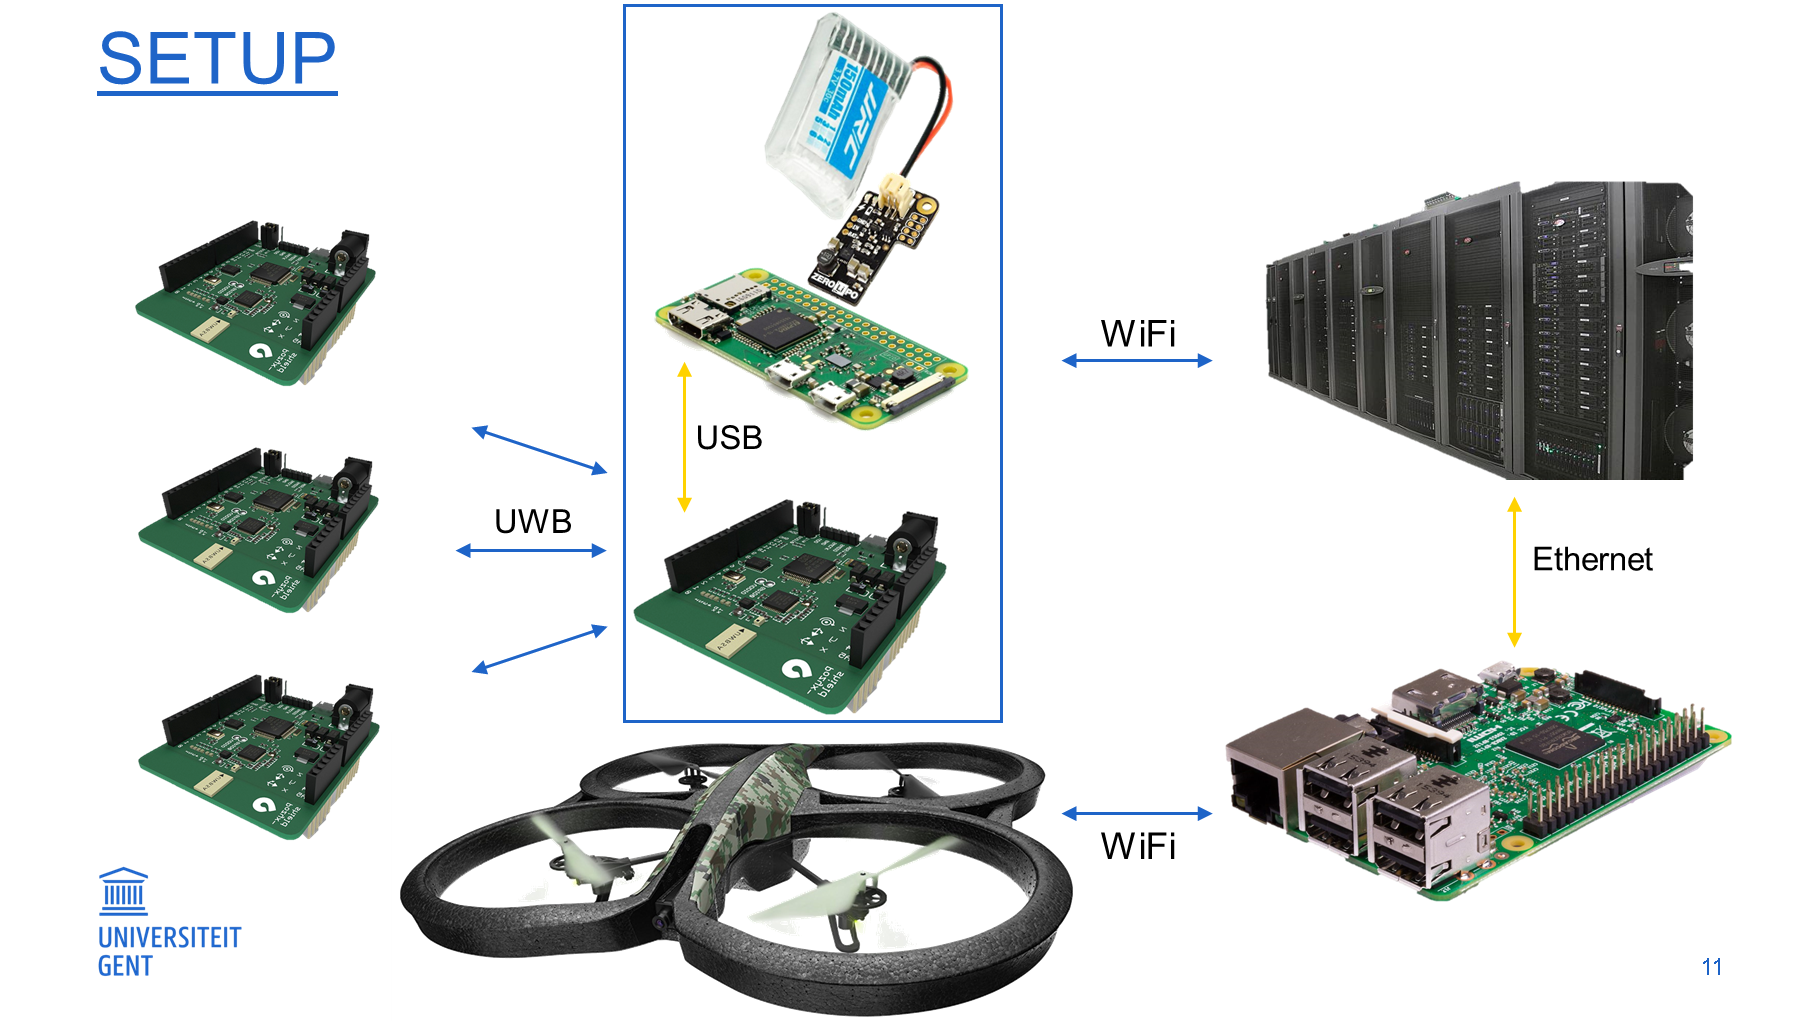
\includegraphics[width=\textwidth]{Setup}
	\caption[Setup]{Hardware setup, aangevuld met protocollen.}
	\label{fig:setup}
\end{figure}

\section{Visualisatie} \label{sec:visualization}
Unity\footnote{\url{https://unity3d.com/}}.